\chapter{Background Studies}
\label{chap:back}

\textit{The decay \Bmumumu is a fully leptonic decay with good potential for eliminating many types of the backgrounds. In this chapter parametrisation and estimations for all considered backgrounds are sketched. A quick summary of all backgrounds that passed the stringent selection were provided in~\autoref{bkgquick}.}

In this chapter summary of considered backgrounds is provided where combinatorial background is described in~\autoref{combiback}, misidentified background in~\autoref{misidprocedure}, different classes of partially reconstructed background are considered in~\autoref{partrecobak} and finally rare and resonant backgrounds considered in~\autoref{rareandreso}.

\section{Combinatorial Background}
\label{combiback}
Combinatorial background comes around as a random combination of tracks from different $b$-decay chains. The usual method at \gls{LHCb} of estimating the amount and the shape of this background include extrapolation from the upper mass data sideband to the signal region. In this case the upper mass sideband is defined as $M_{\rm{B_{corr}}} > 5500 \mevcc$ and the signal region is defined to be $ 4500 \mevcc <M_{\rm{B_{corr}}} < 5500 \mevcc$. The characteristic shape for this background can be described by exponential function up to certain point, where this point is the primary discussion of this section. Since tight selection resulted in low-statistics data samples the extrapolation from upper mass sideband introduces a big uncertainty on the exponential constant and cannot be used to estimate the correct shape and yield of this background. What can be done, however, is to assume the exponential shape for combinatorial component and let the exponential constant be a floating parameter in the data fit. This method for estimation of the combinatorial component will be mentioned in signal data mass fits~\autoref{sigpara}. In the rest of this section exponential parametrisation of this background between $4000 \mevcc <M_{\rm{B_{corr}}} < 7000 \mevcc$ is motivated. This is important as the final fitting region was chosen in such a way as to make sure that combinatorial background is exponential in this entire fitting region. 

Apart from the nominal upper mass data sideband sample, two other samples are analysed as proxies for this type of background. Despite the fact that these samples are also scarcely populated they are studied altogether to determine in which mass regions the combinatorial background can be considered exponential. Firstly, same sign data sample was studies (the same sample as in~\autoref{cloniatkos}), where this sample consists of $\mu^{+} \mu^{+} \mu^{+} \nu$ events passing all selection up to MVA selection to have sufficient statistics. Secondly an inclusive $b\bar{b}$ simulation sample consisting of events where two muons with $p > 3$ \gevc are required to be present alongside  with a third muon. On the top these events have to satisfy all the stripping selection outlined in~\autoref{tab:stripcutsB}.

As seen in~\autoref{fig:bbarcombi}(b)(c), the exponential component stops rising at $M_{\rm{B_{corr}}} = 4000 \mevcc$. Hence the choice of fitting region $4000 \mevcc<M_{\rm{B_{corr}}}<7000\mevcc$.

\begin{figure}[H]
\center
\includegraphics[width = 0.33\textwidth]{bkg/combi/nicenewANAcombiUMSB_WITHPULL_new.pdf}\put(-70,100){(a)}%
\includegraphics[width = 0.33\textwidth]{bkg/combi/nicenewANAcombi3same_WITHPULL_new.pdf}\put(-70,100){(b)}%
\includegraphics[width = 0.33\textwidth]{bkg/combi/nicenewANAcombi_WITHPULL_new.pdf}\put(-70,100){(c)}%
	\caption{(a) Fit to upper mass side band just before application of MVA selection. (b) Fit to $\mu^{+}\mu^{+}\mu^{+}\nu$ same sign sample. (c) Fit to $b\bar{b}$ sample with exponential function. In (b)(c), exponential description is not correct below $4000 \mevcc$. All plots contain exponential constants.}
\label{fig:bbarcombi}
\end{figure}

This background is heavily suppressed with dedicated MVA selection described in~\autoref{CombiBDTsel}.


\section{MisID type background}
\label{misidprocedure}
MisID background is one of the most prominent backgrounds that is expected to be present. This type of background proceeds mostly via cascade decays, where $B^{+} \rightarrow (\bar{D^{0}} \rightarrow h X \mu^{-} \nu) \mu^{+} \nu$ and then $h\in[K^{+},\pi^{+}]$ are misidentified as muons. The contributions from decays where two muons are correctly identified as muons and third track is consistent with proton passing all the selection is also considered, however this contribution is very limited. 

As discussed in~\autoref{bkgquick} there are two possibilities for the charge for the misidentified background. In one case the sign of the misidentified particle agrees with the sign of the mother $B$, \textit{SS misID} background. The opposite case is denoted as \textit{OS misID} decays, which arises less often as it requires decays with more additional particles. These two types of backgrounds are studied using data-driven method described below. Finally, also double misID employing same data-driven methods was studied, where there are two hadrons misidentfied as muons, however, the double misID contribution proved to be insignificant.


To determine the amount and the shape of the misID background, data sample with the same selection as for the signal sample is obtained with one marginal difference - \textbf{no \gls{PID} cut} on one muon, either positive or negative. As the muon misID rate is different for pions and kaons~\cite{LHCb-DP-2013-001}, the species of the hadron, $h$ must be determined at first. The strategy for this purpose is to isolate the hadron into separate hadron \gls{PID} regions, and to determine the cross-feed of one region into the other. For this, an iterative procedure as shown in \autoref{fig:misidproc} is applied ignoring insignificant proton cross-feed. This iterative procedure hence splits the misidentified data sample into \gls{PID} regions, where the hadron candidate is consistent with the kaon, pion and proton hypotheses. For this procedure, probabilities of identifying a given species with given \gls{PID} requirement are taken from dedicated control samples in \texttt{PIDCalib} package \cite{Anderlini:2202412} discussed in~\autoref{extraction}. The \gls{PID} performance is highly dependant on kinematic properties of the misidentified particle and hence the estimation is performed in bins of momentum $p$ and pseudorapidity $\eta$.
At the beginning of the procedure, the number of misidentified events of given species is assumed to be zero, and the
cross-feed between regions is calculated assuming that the pion, kaon and protons regions are pure pions, kaons and protons.
This procedure then corrects the distributions by taking into the account this initial cross-contamination.
This procedure is repeated until the number of total misidentified particles does not change significantly from one iteration to another.

\begin{figure}[h]
  \begin{center}
    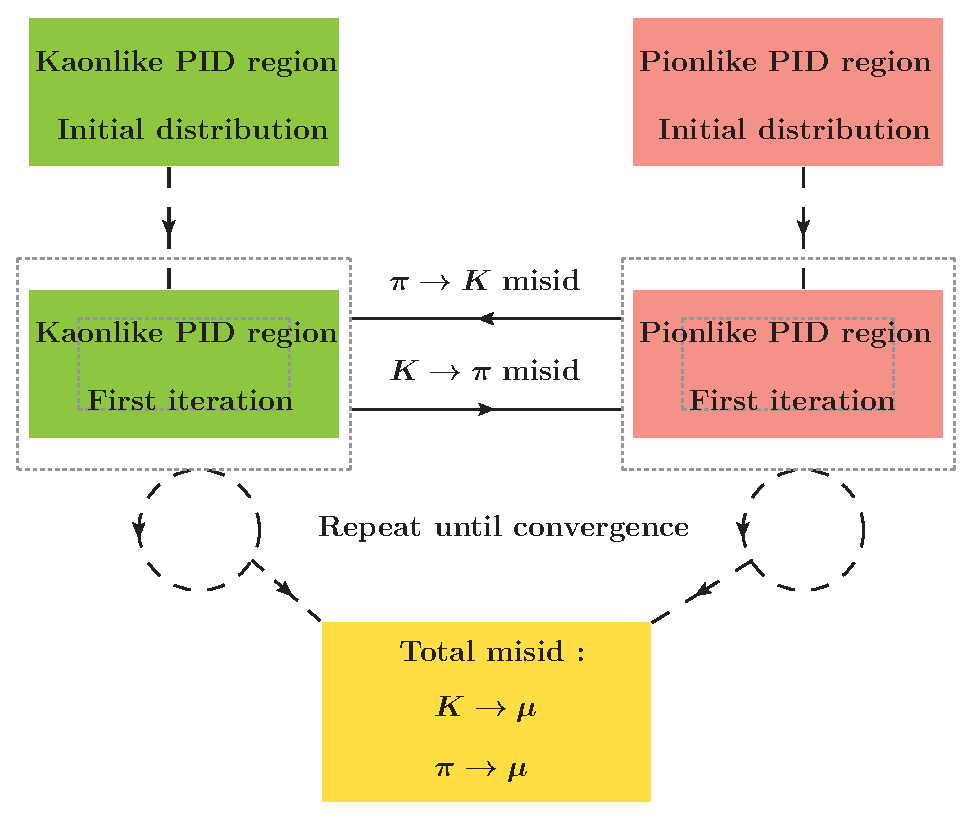
\includegraphics[width=0.6\linewidth]{bkg/misid/misid_att_3}%\put(-32,133){(a)}
    \vspace*{-0.5cm}
  \end{center}
  \caption{
    Diagram of the iterative procedure to establish contamination from decays where pion and kaon are misidentified for muon.
    }
  \label{fig:misidproc}
\end{figure}



Once the cross-feed between the different hadron species has been taken into account, the final step is to calculate the probability for
a specific hadron to pass the stringent muon \gls{PID} requirements applied in the analysis. The presence of the two real muons in the $\mumu h X$
background increases probability to misidentify the hadron as a muon, mainly due to sharing of hits in the muon stations. Therefore the hadron misID probability is obtained from a dedicated control sample designed to emulate the topology of the mis-identified background,
 $B^{0} \rightarrow J/\psi(\rightarrow \mu^{+} \mu^{-}) K^{*}(\rightarrow \underline{K^{+} \pi^{-}})$, as shown in~\autoref{ratiatkos}.

%To determine the amount and the shape of the misID background data sample, same selection as for the signal sample is applied apart from \texttt{no \gls{PID} cut} on one muon, either positive or negative. The stripping selection for this sample is similar but with \texttt{no \gls{PID} cut} for the misidentified muon (SS or OS), see~\autoref{tab:misidbackground}.

This process can be summarized mathematically in a following way:

\begin {itemize}
\item The proton-, pion- and kaon-like regions are defined in~\autoref{tab:misidregions}.

\begin{table}[ht]
\begin{center}
\begin{tabular}[t]{ l  l }
\toprule
Region & PID cuts  \\ \hline
Proton-like & \texttt{DLLp}  > 5, \texttt{DLLp} - \texttt{DLLK} > 5 \\
Kaon-like & \texttt{DLLK} > 0, \texttt{DLLp} - \texttt{DLLK} < 5 \\
Pion-like &  \texttt{DLLK} < 0, \texttt{DLLp} < 5 \\ \bottomrule
\end{tabular}
\end{center}
\caption{Species region definitions.}
\label{tab:misidregions}
\end{table}

%To estimate the shape of the background and size of it following procedure is applied:
%\begin {itemize}
%\item Subdivide
\item ID efficiencies are obtained from \texttt{PIDCalib} in bins of $p$, $\eta$ for all three regions.
\item MisID efficiencies are obtained from the specific calibration sample compensating having two other muons in the sample in~\autoref{ratiatkos} in the bins of $p$, $\eta$.
%Basic misID efficiencies are obtained for following cuts: \texttt{Particle\_(IsMuon==1.0) \&\& (DLLmu > 0.0) \&\& ((DLLmu - DLLK) > 0.0) \&\& (nShared==0)} as these are applied in stripping and selection.
%\item Some of the entries in the tuples are outside of default bins of \texttt{PIDCalib}/Calibration samples. For events below $p<3\gevc$, these are not considered and cut out (in signal data this is done by requiring \texttt{isMuon}). For events $p>100\gevc$, the same id/misID probability as the last bin is assigned.
%\item Some bins of \texttt{PIDCalib}/Calibration samples yield probabilities that are unphysical. These bins have either negative probabilities or probabilities above 1 (can arise due to $Splot$ technique used in \texttt{PIDCalib}). For bins with negative probabilities, probability is set to 0.00001. For bins with probability above 1 are set 1. And for bins which were not populated, the value from neighbouring bin was used. Remark: negative bins only appear for proton misID. As it will be shown in the misID fit section there is very small contribution from protons so there is no bias for the pion/kaon samples. The misID probabilities for different years will be discussed and shown in~\autoref{fig:JpsiKstWeights} and as it can be seen there are no negative bins.
\item In order to account for cross-contamination between the kaon and pions species the following procedure is applied:

\begin{itemize}

\item The data in each region is binned to obtain two dimensional $N(p, \eta)$ distributions, where $p$ is momentum and $\eta$ is pseudorapidity. The true kinematical distributions for kaons and pions are given by
\begin{equation}
n(p, \eta )^{0}_{\pi/K} = \frac{N(p, \eta )_{\pi/K}}{\epsilon(p,\eta )_{\pi/K}}.
\end{equation}
where $\epsilon(p,\eta)_{\pi/K}$ are efficiencies obtained from \texttt{PIDCalib} tables.

\item To correct for the cross-feed between pion and kaon regions, following algorithm which corrects the original distribution is applied:

\begin{equation}
n(p, \eta)^{i+1}_{\pi}=\frac{N(p, \eta)_{\pi}-M(p, \eta)_{K \rightarrow \pi} n(p, \eta)^{i}_{K}}{\epsilon(p,\eta)_{\pi}},
\end{equation}
\begin{equation}
n(p, \eta)^{i+1}_{K}=\frac{N(p, \eta)_{K}-M(p, \eta)_{\pi \rightarrow K} n(p, \eta)^{i}_{\pi}}{\epsilon(p,\eta)_{K}}.
\end{equation}

Here, $n(p, \eta)^{i}_{\pi}$  $n(p, \eta)^{i}_{K}$ together with the misID binned efficiencies $M(p, \eta )_{K \rightarrow \pi}$ and $M(p, \eta)_{\pi \rightarrow K}$ are estimating the-cross contamination between two regions.

%\item The next order distributions $n(p, \eta)^{i+1}_{\pi/K}$ are obtained by correcting the original distributions with the cross-contamination and then correcting for the ID binned efficiency.

\item At each iteration, the total number of misID particles of the type $\pi \rightarrow \mu$ and $K \rightarrow \mu$ events are given by
\begin{equation}
\sum_{p,\eta} n(p, \eta)^{i}_{\pi} M(p, \eta)_{\pi\rightarrow\mu} 
\end{equation}
\begin{equation}
\sum_{p,\eta} n(p, \eta)^{i}_{K} M(p, \eta)_{K\rightarrow\mu}
\end{equation}
\item This procedure is repeated until the change in total misID between iterations is less than 0.1\%. Typical number of iterations depends on the size of the sample. For big samples the convergence is achieved after two or three iterations. For small samples this is achieved after six iterations on average.

\item For each event in both kaon-like and pion-like sample, $w_{cross-feed}$ = probability of being misidentified particle including the cross-contamination correction is 
	calculated 
\begin{equation}
w_{cross-feed}=\frac{n(p, \eta)^{final}_{\pi} \times M(p, \eta)_{\pi\rightarrow\mu}}{{N(p, \eta)}^{0}_{\pi}},
\end{equation}
\begin{equation}
w_{cross-feed}=\frac{n(p, \eta)^{final}_{K} \times M(p, \eta)_{K\rightarrow\mu}}{{N(p, \eta)}^{0}_{K}}.
\end{equation}
\end{itemize}

\item The number of misidentified events and the shape are obtained by reweighting the pion-like and kaon-like datasets by the $w_{cross-feed}$. 
	
%	The difference between unweighted, weighted by PID efficiencies with no cross-feed, and weighted with cross-feed distributions can be seen in~\autoref{fig:misidtemp}.
\end{itemize}

Examples of misID distributions with unweighted, weighted by probability with no cross-feed correction, and weighted with cross-feed correction can be seen in~\autoref{fig:misidtemp} for the \textit{SS misID} and ~\autoref{fig:misidtempOS} for the \textit{OS misID}. These are the misID distributions before misid BDTs are applied, which minimize the contamination of this background as discussed in~\autoref{misidbdt}. 

\begin{figure}[H]
\center
\includegraphics[width = 0.9\textwidth]{/bkg/misid/example/compare_misid_modifiedandcutnSharednewData_B23MuNu_MisidSS_Run1_mu3isNotMuon_mu3inMuonAcc_trigger_Jpsi_mu1nShared_mu2nShared_qmincut_KaonPID__NEW.pdf}\put(-300,133){(a)}\put(-50,133){(b)}
\newline
\includegraphics[width = 0.9\textwidth]{/bkg/misid/example/compare_misid_modifiedandcutnSharednewData_B23MuNu_MisidSS_Run1_mu3isNotMuon_mu3inMuonAcc_trigger_Jpsi_mu1nShared_mu2nShared_qmincut_PionPID__NEW.pdf}\put(-300,133){(c)}\put(-50,133){(d)}
%\newline
%\includegraphics[width = 0.9\textwidth]{/bkg/misid/example/compare_misid_modifiedandcutnSharednewData_B23MuNu_MisidOS_Run1_mu2isNotMuon_mu2inMuonAcc_trigger_mu1nShared_mu3nShared_qmincut_KaonPID__NEW.pdf}\put(-300,133){(e)}\put(-50,133){(f)}
%\newline
%\includegraphics[width = 0.9\textwidth]{/bkg/misid/example/compare_misid_modifiedandcutnSharednewData_B23MuNu_MisidOS_Run1_mu2isNotMuon_mu2inMuonAcc_trigger_mu1nShared_mu3nShared_qmincut_PionPID__NEW.pdf}\put(-300,133){(g)}\put(-50,133){(h)}
\caption{Examples of distributions where misID procedure is applied to obtain yields and shapes for Run \Rn{1} before misID BDT was applied. On the left, unweighted misID distributions (black), weighted with no cross-feed misID distributions (blue) and weighted misID distributions with cross-feed (red) for (a) kaon SS (c) pion SS . On the right, only weighted misID distributions for Run \Rn{1} (b) kaon SS (d) pion SS are shown together with the yield estimates. These shapes are obtained after combinatorial BDT was applied, but before misid BDT was applied. Total yields need to be multiplied by 100 to counteract the prescale that was applied on this data.}
\label{fig:misidtemp}
\end{figure}


\begin{figure}[H]
\center
%\includegraphics[width = 0.9\textwidth]{/bkg/misid/example/compare_misid_modifiedandcutnSharednewData_B23MuNu_MisidSS_Run1_mu3isNotMuon_mu3inMuonAcc_trigger_Jpsi_mu1nShared_mu2nShared_qmincut_KaonPID__NEW.pdf}\put(-300,133){(a)}\put(-50,133){(b)}
%\newline
%\includegraphics[width = 0.9\textwidth]{/bkg/misid/example/compare_misid_modifiedandcutnSharednewData_B23MuNu_MisidSS_Run1_mu3isNotMuon_mu3inMuonAcc_trigger_Jpsi_mu1nShared_mu2nShared_qmincut_PionPID__NEW.pdf}\put(-300,133){(c)}\put(-50,133){(d)}
%\newline
\includegraphics[width = 0.9\textwidth]{/bkg/misid/example/compare_misid_modifiedandcutnSharednewData_B23MuNu_MisidOS_Run1_mu2isNotMuon_mu2inMuonAcc_trigger_mu1nShared_mu3nShared_qmincut_KaonPID__NEW.pdf}\put(-300,133){(a)}\put(-50,133){(b)}
\newline
\includegraphics[width = 0.9\textwidth]{/bkg/misid/example/compare_misid_modifiedandcutnSharednewData_B23MuNu_MisidOS_Run1_mu2isNotMuon_mu2inMuonAcc_trigger_mu1nShared_mu3nShared_qmincut_PionPID__NEW.pdf}\put(-300,133){(c)}\put(-50,133){(d)}
\caption{Examples of distributions where misID procedure is applied to obtain yields and shapes for Run \Rn{1} before misID BDT was applied. On the left, unweighted misID distributions (black), weighted with no cross-feed misID distributions (blue) and weighted misID distributions with cross-feed (red) for (a) kaon OS (c) pion OS. On the right, only weighted misID distributions for Run \Rn{1} (b) kaon OS (d) pion 0S are shown together with the yield estimates.  These shapes are obtained after combinatorial BDT was applied, but before misid BDT was applied. Total yields need to be multiplied by 100 to counteract the prescale that was applied on this data.}
\label{fig:misidtempOS}
\end{figure}


\section{Partially Reconstructed Background}
\label{partrecobak}
Partially reconstructed background can occur by missing or misidentifying one or more particle tracks in the decay. The common feature for this type of backgrounds is that the corrected or reconstructed mass of the $B$ will be lower than in the signal case.

In order to estimate both the shape and the size of the partially reconstructed backgrounds, one of the most dangerous example is studied: $B^+ \rightarrow (D^0 \rightarrow K^- \pi^+ \mu^{+} \mu^{-})\mu \nu$. The expected $\mathcal{B}(\pr)$ is obtained by amalgamating $\mathcal{B}(D^{0} \rightarrow K^+ \pi^- \mu^+ \mu^{-}) = (4.17\pm0.12\pm0.40)\times 10^{-6}$\cite{Aaij:2015hva} and $\mathcal{B}(B^{+} \rightarrow D l^{+} \nu X) = (9.8 \pm 0.7)\times 10^{-2}$ \cite{Patrignani:2016xqp} yielding $\mathcal{B}(\pr) \approx (4.10\pm0.50)\times 10 ^{-7}$.

The shape of this background is investigated with inclusive simulation samples containing also higher excited resonances of $D^{*0}, D_{2}^{*0}$, and so on. This simulation has one imperfection: it has two charged pions rather than muons coming from the $D^{0}$ decay, which are reconstructed as signal. In this study the effect of missing particles on the corrected mass shape is investigated hence these two pions become good proxies for the muons given the muon and pion have very similar mass. The only problem that could arise is if the selection efficiency was not constant as a function of the dipion mass, $M(\pi^{+}\pi^{-})$, as this would lead to shaping of the background, potentially underestimating the contributions from the resonant $\omega$ and $\rho$ region, which are present with the two muons. 

For this reason all muon cuts from selection apart from the \gls{PID} are also applied to pions. Relative efficiency ratios including all the efficiencies after MVA stage are obtained, where for signal the total selection efficiency is $\varepsilon^{total}_{\Bmumumu}=(2.63 \pm 0.03)\times 10^{-3}$ and for partially reconstructed background $\epsilon^{total}_{\pr}=(6.82 \pm 0.07)\times 10^{-4}$. Assuming the branching fractions for $\mathcal{B}(\Bmumumu) = 1\times10^{-8}$ and for $\mathcal{B}(\pr ) = (4.10\pm0.50)\times10^{-7}$, relative contamination between signal and partially reconstructed background results in~\autoref{fig:expectedinter}(a). 

To check the fact that there is no dangerous shaping of the background using this particular proxy simulation sample the full selection efficiency in bins of dipion mass is plotted. The efficiency flatness shown in~\autoref{fig:expectedinter}(b) means that this selection does not have model dependence and hence it is safe to use for shape estimates for the partially reconstructed backgrounds.
%not exact because of minq contamination

\begin{figure}[H]
\centering
\includegraphics[width = 0.5\textwidth]{bkg/pr/variableBplus_Corrected_MassPartRecoScaled2012_0_102_supernice.pdf}\put(-50,70){(a)}
\includegraphics[width = 0.47\textwidth]{bkg/pr/SelectionEfficiency_invmu1andmu2_PARTRECOMC_special.pdf}\put(-50,70){(b)}
	\caption{(a) Signal and partially reconstructed background distributions scaled to their expected ratio after full MVA selection assuming following branching fractions: $\mathcal{B}(\Bmumumu ) = 1\times10^{-8}$ and $\mathcal{B}(\pr ) = (4.10\pm0.50)\times10^{-7}$. (b) Full selection efficiency as a function of invariant mass of the proxy pions is constant.}
\label{fig:expectedinter}
\end{figure}


The most powerful part of selection that eliminates this part of the background is isolation as partially reconstructed background decay had usually has more tracks. In order to estimated contamination in the final fit, normalisation with respect to \bjpsimumuk is used as shown in~\autoref{finfitpr}.

\subsection{Partially Reconstructed Backgrounds, where \mb{D^{0} \rightarrow \eta / \eta' X}, and \mb{\eta / \eta' \rightarrow \mu \mu \gamma}}
\label{etasec}
In the previous partially reconstructed sample, the background that proceed via $\eta/\eta'$ from $D$ resonance is not considered, as it is not part of the inclusive simulation. The selection efficiency of such decays is expected to have very similar values as in the partially reconstructed sample proxy, because the reconstructed particles are the same.

In this section, the total estimate for the branching fraction of partially reconstructed backgrounds proceeding via $\eta/\eta'$ from $D$ resonances is computed. Full inclusive rate $\mathcal{B} (D^{0} \rightarrow \eta / \eta' X)$ is $ \sim 10 \%)$. However, the most relevant decay chains are the ones where the mass of the missed particle is small. This is because if only light particle is missed, the shape of corrected mass of partially reconstructed background comes closest to the signal region. Such decay chains are considered in~\autoref{tab:etacont}.

It can be seen that total cumulative contribution is much smaller then the one considered with $D^{0}\rightarrow K^{+} \pi^{-} \mu^{+} \mu^{-}$, where $\mathcal{B}(D^0 \rightarrow K \pi^+ \mu^{+} \mu^{-}) = (4.17\pm0.12 \rm{(stat)}\pm 0.40 \rm{(syst)})\times 10^{-6}$\cite{Aaij:2015hva}. No further consideration hence is necessary for this type of decay.

\begin{table}[ht]
\begin{center}
\begin{tabular}{ l  c  c }

\toprule
	Process & $\mathcal{B}$ & Contribution to $\mathcal{B}(D^{0} \rightarrow (\eta / \eta'\rightarrow \mu \mu \gamma) X)$ \\
\hline

$\mathcal{B}(\eta \rightarrow \mu \mu \gamma)$ & $(3.10\pm0.40)\times 10 ^{-4 }$ & -  \\
$\mathcal{B}(\eta' \rightarrow \mu \mu \gamma)$ & $(1.08\pm0.27)\times 10 ^{-4 }$ & -  \\
\hline
$\mathcal{B}(D^{0} \rightarrow \eta' \pi^{0})$ & $(9.10\pm1.40)\times 10 ^{-4 }$ & $(9.80\pm2.90)\times 10 ^{-8 }$ \\
$\mathcal{B}(D^{0} \rightarrow \eta' \pi^{+} \pi^{-})$ & $(4.50\pm1.70)\times 10 ^{-4 }$ & $(4.90\pm2.20)\times 10 ^{-8 }$ \\
$\mathcal{B}(D^{0} \rightarrow 2\eta )$ & $(1.70\pm0.02)\times 10 ^{-3 }$ & $(5.30\pm0.70)\times 10 ^{-7 }$ \\
$\mathcal{B}(D^{0} \rightarrow 2\eta )$ & $(1.70\pm0.02)\times 10 ^{-3 }$ & $(5.30\pm0.70)\times 10 ^{-7 }$ \\
$\mathcal{B}(D^{0} \rightarrow \underline{\eta} \eta' )$ & $(1.06\pm0.27)\times 10 ^{-3 }$ & $(3.30\pm0.90)\times 10 ^{-7 }$ \\
$\mathcal{B}(D^{0} \rightarrow \eta \underline{\eta}' )$ & $(1.06\pm0.27)\times 10 ^{-3 }$ & $(1.10\pm0.40)\times 10 ^{-7 }$ \\
$\mathcal{B}(D^{0} \rightarrow \eta \phi)$ & $(1.40\pm0.50)\times 10 ^{-4 }$ & $(4.30\pm1.60)\times 10 ^{-8 }$ \\
\hline
Total &  - &$(1.69\pm0.15)\times 10 ^{-6 }$ \\
\bottomrule
\end{tabular}
\end{center}
\caption{Contribution to total $D^{0} \rightarrow (\eta / \eta'\rightarrow \mu \mu \gamma) X$ rate made from all the considered decays above. In total, this cumulative contribution is approximately three times smaller than $D^{0}\rightarrow K^{+} \pi^{-} \mu^{+} \mu^{-}$. All the branching fractions are obtained from \cite{Patrignani:2016xqp}.}
\label{tab:etacont}
\end{table}

\subsection{Partially Reconstructed \mb{B \rightarrow \eta (') V} Backgrounds}
The backgrounds with $\eta(')$ resonances from partially reconstructed decays that proceed via $D$ were considered in previous~\autoref{etasec}. In this section backgrounds with $\eta(')$ along with vector resonances $\omega$/$\rho$ coming directly from $B$ are estimated. The total branching fractions for these processes are listed in~\autoref{tab:ed} and since they are very small this type of background is discarded and will not be considered further.

\begin{table}[ht]
\begin{center}
\begin{tabular}{ l  c }
\toprule
Process & $\mathcal{B}$  \\
\hline
$\mathcal{B}(B^{0} \rightarrow \omega \eta')$ & $(1.00\pm0.50)\times 10 ^{-6 }$ \\
$\mathcal{B}(B^{0} \rightarrow \rho \eta')$ &  $<$$5 \times 10 ^{-7}$  \\
$\mathcal{B}(B^{0} \rightarrow  \omega  \eta )$ & $(9.00\pm4.00)\times 10 ^{-7 }$ \\
$\mathcal{B}(B^{0} \rightarrow \rho \eta )$ & $<$ $5 \times 10 ^{-7}$   \\
\hline
$\mathcal{B}(\eta \rightarrow \mu \mu \gamma)$ & $(3.10\pm0.40)\times 10 ^{-4 }$ \\
$\mathcal{B}(\eta' \rightarrow \mu \mu \gamma)$ & $(1.08\pm0.27)\times 10 ^{-4 }$  \\
\hline
$\mathcal{B}(\rho \rightarrow \mu \mu)$ & $(4.55\pm0.28)\times 10 ^{-5 }$  \\
$\mathcal{B}(\omega \rightarrow \mu \mu)$ & $(9.00\pm3.10)\times 10 ^{-5 }$  \\
\hline
Process & Contribution to $B^{0} \rightarrow (\eta(')\rightarrow \mu \mu \gamma) (\rho(\omega)\rightarrow \mu \mu)$ \\
\hline
$\mathcal{B}(B^{0} \rightarrow (\omega \rightarrow \mu \mu) (\eta \rightarrow \mu \mu \gamma))$ &$(7.10\pm1.00)\times 10 ^{-15 }$ \\
$\mathcal{B}(B^{0} \rightarrow (\omega \rightarrow \mu \mu) (\eta'\rightarrow \mu \mu \gamma))$ &$(2.50\pm0.60)\times 10 ^{-15 }$ \\
$\mathcal{B}(B^{0} \rightarrow (\rho \rightarrow \mu \mu) (\eta \rightarrow \mu \mu \gamma))$ & $<$$(2.50\pm1.40)\times 10 ^{-14 }$ \\
$\mathcal{B}(B^{0} \rightarrow (\rho \rightarrow \mu \mu) (\eta'\rightarrow \mu \mu \gamma))$ & $<$$(1.00\pm0.60)\times 10 ^{-14 }$ \\
\hline
Total  & $ <$ $(4.50\pm1.60)\times 10 ^{-14 }$ \\
\bottomrule
\end{tabular}
\end{center}
\caption{Different and total contribution to $B^{0} \rightarrow \eta(') \rho(\omega)$. All the branching fractions are obtained from \cite{Patrignani:2016xqp}.}
\label{tab:ed}
\end{table}


\section{Rare and resonant \mb{B^{+} \rightarrow \pi^{+} / K^{+} \mu^{-} \mu^{+}} backgrounds}
\label{rareandreso}
The resonant backgrounds arising through $B^{+} \rightarrow (J/\psi \rightarrow \mu^{-} \mu^{+}) X^{+}$ and $B^{+} \rightarrow (\psi(2S) \rightarrow \mu^{-} \mu^{+}) X^{+}$ decay chains are eliminated because of the $c\bar{c}$ veto as discussed in~\autoref{qsqchoice}.

It is, however, necessary to evaluate the impact of the rare equivalent of this background, namely \bmumupi decays, where $\pi^{+}$ is misidentified as muon. The $\mathcal{B}(\bmumupi)=1.79\pm0.23\times 10^{-8}$\cite{Patrignani:2016xqp}. The contribution of this background is accounted for in the~\autoref{misidprocedure}, but it is crosschecked as this particular background peaks just under the corrected mass of $B$. For the same rare decay but with kaon instead, \bmumuk, the mass is expected to be shifted away from this peak because of the higher kaon mass.

In order to establish the severity of this background, \bmumupi simulation for Run \Rn{1} and Run \Rn{2} is reconstructed where the muon mass hypothesis is used for the pion track candidate. This means that energy of this candidate is recalculated. After, the same selection as in the signal case is applied. The expected number of \bmumupi decays after all selection in a given Run can be calculated by normalising to \bjpsimumuk decays. In the end 0.06 (0.03) \bmumupi events are expected in Run \Rn{1} (\Rn{2}) which is negligible given that there are $\sim$ 17 expected signal events with $\mathcal{B}(\Bmumumu)=1\times 10^{-8}$. Hence no further specific action for this background is taken, however, its contribution is directly accounted for in the~\autoref{misidprocedure}.

%\begin{equation}
%	N(\bmumupi)= \frac{N(\bjpsimumuk)}{} \times \frac{\varepsilon^{total}_{\bmumupi}}{\varepsilon^{total}_{\bjpsimumuk}} \times \frac{\mathcal{B}(\bmumupi)}{\mathcal{B}(\bjpsimumuk)}.
%\end{equation}

%info foun in /vols/lhcb/ss4314/final_tuples_analyser_PO_AND_UE/mc/pimumu_mc/normalize_to_jpsik/bin
%why reco factor of 100?


%In this equation the following branching fractions are used: $\mathcal{B}(\bmumupi)=1.79\pm0.23\times 10^{-8}$\cite{Patrignani:2016xqp} and $\mathcal{B}(\bjpsimumuk)=(6.12\pm0.19)\times10^{-5}$) obtained by multiplying $\mathcal{B}(B^{+} \rightarrow J/\psi K^{+}) = (1.026\pm 0.031)\times 10^{-3}$\cite{Patrignani:2016xqp} and $\mathcal{B}(J/\psi \rightarrow \mu^{-} \mu^{+}) = (5.961 \pm0.003) \times 10^{-2}$\cite{Patrignani:2016xqp}. The total selection efficiencies without \gls{PID} are $\varepsilon^{total}_{\bmumupi}=(7.03 \pm 1.13)\times 10^{-6}$ and $\varepsilon^{total}_{\bjpsimumuk}=(5.8\pm0.01)\times10^{-3}$ where the reconstruction and combinatorial BDT efficiency is much lower for the \bmumupi mode. Using the yields obtained in~\autoref{tab:normchannelyields} 0.06 (0.03) \bmumupi events are expected in Run \Rn{1} (\Rn{2}) which is negligible given that there are $\sim$ 17 expected signal events with $\mathcal{B}(\Bmumumu)=1\times 10^{-8}$. Hence no further specific action for this background is taken, however, its contribution is directly accounted for in the~\autoref{misidprocedure}.

\section{Summary}
In conclusion, different backgrounds that can mimic the signal were studied. From all considered backgrounds only combinatorial, misID and partially reconstructed backgrounds have considerable contribution after all the selection and hence need to be modelled. Exact contribution of these three backgrounds is discussed in~\autoref{sigpara}.

